\documentclass[./main.tex]{subfiles}

\begin{document}

\subsection{External Interface Requirements}

\subsubsection{User Interfaces}

The following mockups are made to give an idea of how the user
interfaces should look like after the developing process. The mockups
represent the core services of SafeStreets focusing on the interaction
between the users and the system.

\vfill

\begin{figure}[H]
    \centering
    \begin{minipage}[t]{\mockupsize}
        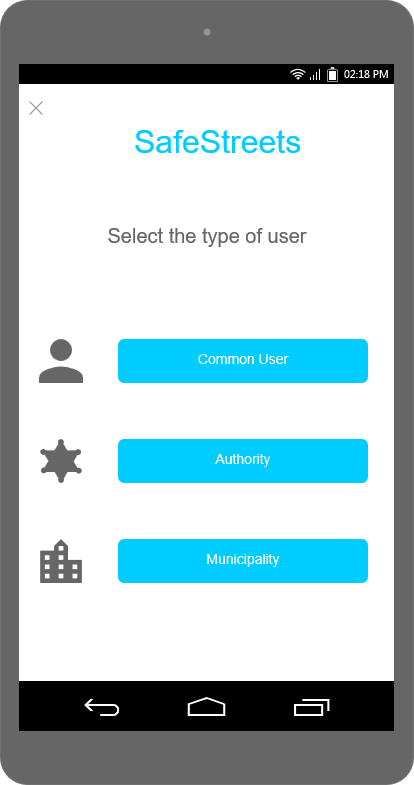
\includegraphics[width=\textwidth]{mockup/choose_user}
        \caption{\protect\raggedright The choice between different types of users.}
    \end{minipage}
    \hfill
    \begin{minipage}[t]{\mockupsize}
        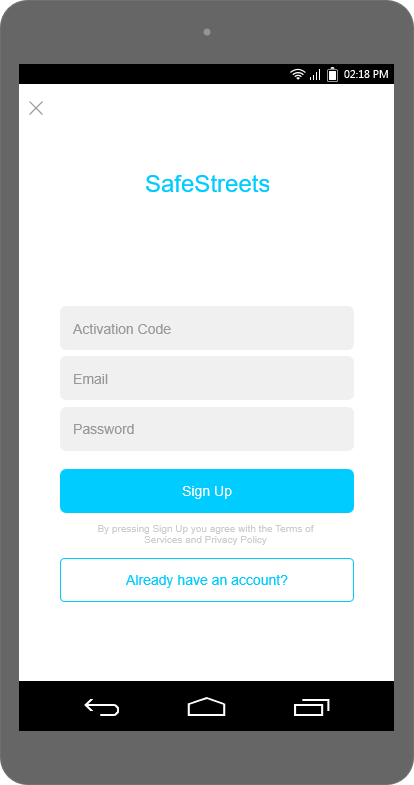
\includegraphics[width=\textwidth]{mockup/sign_up}
        \caption{\protect\raggedright The sign-up process for the municipality user.}
    \end{minipage}
\end{figure}

\vfill
\newpage

\begin{figure}[H]
    \centering
    \begin{minipage}[t]{\mockupsize}
        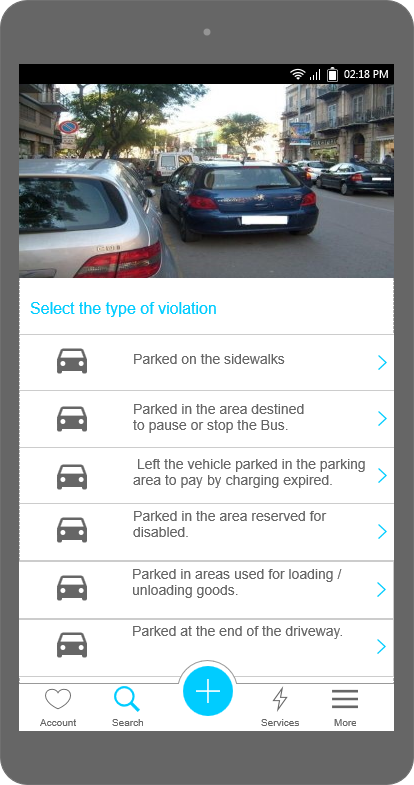
\includegraphics[width=\textwidth]{mockup/select_violation}
        \caption{Selection of the type of violation after a user took a
picture.}
    \end{minipage}
    \hfill
    \begin{minipage}[t]{\mockupsize}
        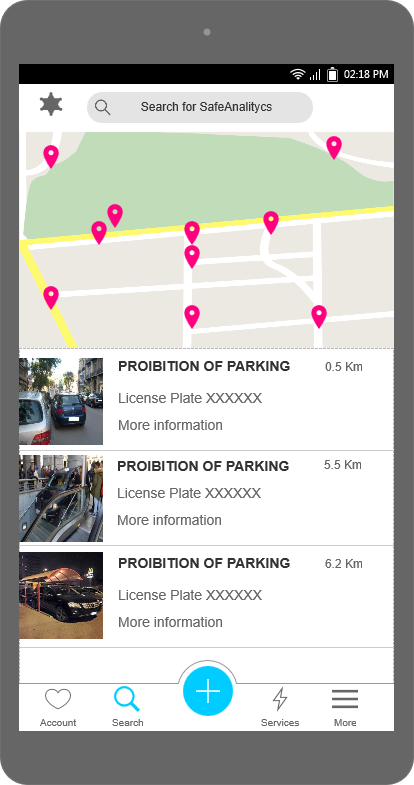
\includegraphics[width=\textwidth]{mockup/get_violations}
        \caption{The result of a query for violations made by an
authority.}
    \end{minipage}
\end{figure}

\begin{figure}[H]
    \centering
    \begin{minipage}[t]{\mockupsize}
        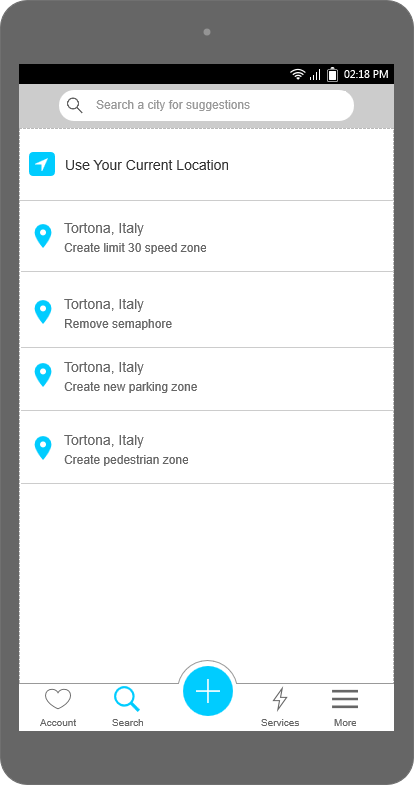
\includegraphics[width=\textwidth]{mockup/get_suggestions}
        \caption{The result of a query using SafeSuggestions.}
    \end{minipage}
\end{figure}

\newpage

\subsubsection{Hardware Interfaces}

The system does not provide any hardware interface.

\subsubsection{Software Interfaces}

The system does not provide any software interface.

\subsubsection{Communication Interfaces}

The system does not provide any communication interface.

\subsection{Functional Requirements}

\subsubsection{Scenarios}

\paragraph{Scenario 1}
Ted Mosby, a very honest architect, is tired of seeing cars parked in
the red zone right in front of his house. He told the problem to some
police agents in the past but nothing happened. He wants to report these
violations again but he doesn't know how to do it. Fortunately, Barney,
a public employee, suggests him to download and use the new SafeStreets
application for reporting violations. After signing up identifying
himself as a common user and inserting the email and password he can
finally report the violation. Mosby just needs to activate the GPS and
the internet connection and take a picture of the violation. He selects
the type of violation from a predefined list. After that, he is asked to
confirm the plate of the violating vehicle. He finally waits for the
outcome of his violation report.

\paragraph{Scenario 2}
Sheldon, a theoretical physicist, is currently studying the complexity
theory. He thinks that in big cities with a huge amount of traffic the
number of traffic violations is much larger than in small cities and
villages. Since Sheldon moved to Milan recently, he wants to know the
areas of Milan with the highest levels of traffic violations to avoid
parking in dangerous places. Sheldon knows about the SafeStreets app. He
logs in inserting his email and password and makes a query for all the
traffic violations reported in the last month in Milan. The results are
anonymized preserving the privacy of the violators and then sent back to
Sheldon. Sheldon can now park in safe areas.

\paragraph{Scenario 3}
Chuck, a policeman, was notified about a stolen car. He gets the idea of
looking for its possible traffic violations, to find it. He uses
SafeAnalytics to retrieve information about it, searching for its
license plate. Chuck discovers that the car is often parked on certain
reserved parking and finds the car in that location.

\paragraph{Scenario 4}
Seamus, the police chief, needs to collect the more money he can from
traffic tickets, to fund the construction of another police station.
Thanks to SafeTickets, he can identify the areas in which more traffic
tickets are generated and focus on those areas.

\paragraph{Scenario 5}
Giovanni, a municipality officer of the city of Milan, is looking for
possible interventions in the city, to improve the mobility of his area.
Giovanni logs in SafeStreets and accesses SafeSuggestions. He is
suggested to build a barrier near the sidewalk in Via Golgi, due to the
frequent parking violations that occur there.

\subsubsection{Common users}

\begin{figure}[H]
\centering
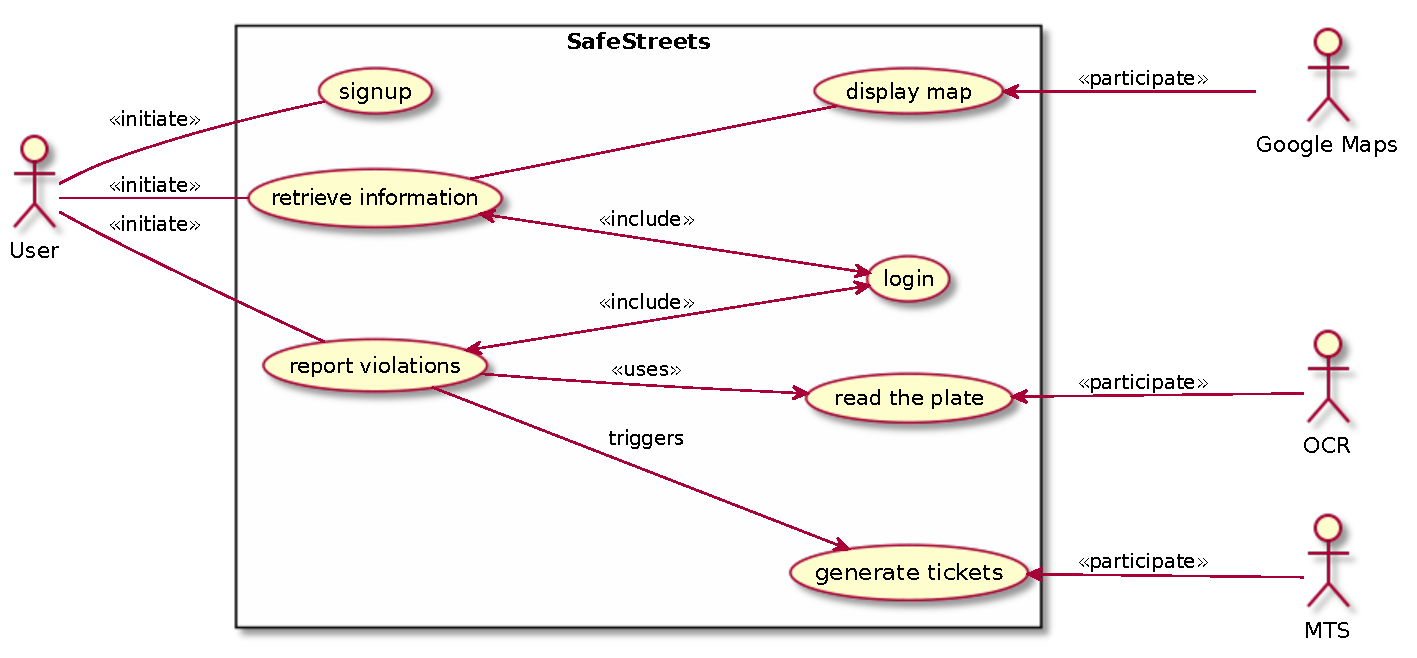
\includegraphics[width=\textwidth]{usecase_common_user.pdf}
\caption{Use cases diagram}
\end{figure}

\begin{table}[H]
\centering
\begin{tabularx}{\textwidth}{|l|X|}
\hline
Name & Sign up\tabularnewline
\hline
Actors &
\begin{itemize}[nosep,leftmargin=*]
\item Common user
\end{itemize}
\tabularnewline
\hline
Entry conditions &
\begin{itemize}[nosep,leftmargin=*]
\item The user opens the app on his smartphone
\end{itemize}
\tabularnewline
\hline
Events flow &
\begin{itemize}[nosep,leftmargin=*]
\item The user clicks on the sign up button
\item The user selects the option to identify himself as a common user
\item The user fills the forms with his email and a password
\item The system confirms his data
\item The system adds the new user to his data
\end{itemize}
\tabularnewline
\hline
Exit conditions &
\begin{itemize}[nosep,leftmargin=*]
\item The users is now registered and his account is registered to the
system
\end{itemize}
\tabularnewline
\hline
Exceptions &
\begin{itemize}[nosep,leftmargin=*]
\item The user has already an account. In this case the system suggests
the user to click the login button instead or to use another email
\end{itemize}
\tabularnewline
\hline
\end{tabularx}
\end{table}

\begin{table}[H]
\centering
\begin{tabularx}{\textwidth}{|l|X|}
\hline
Name & Login\tabularnewline
\hline
Actors &
\begin{itemize}[nosep,leftmargin=*]
\item Common user
\end{itemize}
\tabularnewline
\hline
Entry conditions &
\begin{itemize}[nosep,leftmargin=*]
\item The users opens the app on his device
\item The user has already signed up
\end{itemize}
\tabularnewline
\hline
Events flow &
\begin{itemize}[nosep,leftmargin=*]
\item The users presses the login button
\item The users types the email and the password
\item The system confirms the successful login
\end{itemize}
\tabularnewline
\hline
Exit conditions &
\begin{itemize}[nosep,leftmargin=*]
\item The user is logged in and is able to use the SafeStreets services
\end{itemize}
\tabularnewline
\hline
Exceptions &
\begin{itemize}[nosep,leftmargin=*]
\item The user types the wrong email or password. In both cases the system
sends an error to the user asking him to try the email password
combination again
\end{itemize}
\tabularnewline
\hline
\end{tabularx}
\end{table}

\begin{table}[H]
\centering
\begin{tabularx}{\textwidth}{|l|X|}
\hline
Name & Report a violation\tabularnewline
\hline
Actors &
\begin{itemize}[nosep,leftmargin=*]
\item Common user
\item OCR
\end{itemize}
\tabularnewline
\hline
Entry conditions &
\begin{itemize}[nosep,leftmargin=*]
\item The user has already done the login
\end{itemize}
\tabularnewline
\hline
Events flow &
\begin{itemize}[nosep,leftmargin=*]
\item The user takes a picture of the traffic violation
\item The required metadata are automatically added to the picture
\item The user selects the type of violation from a list of violations
\item The picture is sent to the OCR software to automatically scan and
read the plate
\item After receiving the plate from the OCR, the system asks the user to
confirm the plate of the violation vehicle
\item After the confirmation the system checks if the new violation is
equivalent to an already stored one
\item The system checks the integrity of the report
\item The systems stores the violation report if and only if the previous
equivalence check returned a negative result and the integrity test was
positive
\end{itemize}
\tabularnewline
\hline
Exit conditions &
\begin{itemize}[nosep,leftmargin=*]
\item The user receives a notification about the outcome of its violation
\end{itemize}
\tabularnewline
\hline
Exceptions &
\begin{itemize}[nosep,leftmargin=*]
\item If the OCR is not able to read the plate then the system sends an
error to the user and asks him to repeat the procedure
\end{itemize}
\tabularnewline
\hline
\end{tabularx}
\end{table}

\begin{table}[H]
\centering
\begin{tabularx}{\textwidth}{|l|X|}
\hline
Name & Generate tickets\tabularnewline
\hline
Actors &
\begin{itemize}[nosep,leftmargin=*]
\item SafeStreets
\item MTS
\end{itemize}
\tabularnewline
\hline
Entry conditions &
\begin{itemize}[nosep,leftmargin=*]
\item The system has validated and stored a new traffic violation report
\end{itemize}
\tabularnewline
\hline
Events flow &
\begin{itemize}[nosep,leftmargin=*]
\item The system forwards the violation report to MTS
\item MTS generates tickets from the violation report
\item MTS sends the results to SafeStreets
\end{itemize}
\tabularnewline
\hline
Exit conditions &
\begin{itemize}[nosep,leftmargin=*]
\item The system stores data about issued tickets and builds statistics
from that data
\end{itemize}
\tabularnewline
\hline
Exceptions &
\begin{itemize}[nosep,leftmargin=*]
\item If MTS is not able to generate the tickets then and error is sent to
SafeStreets and no data about issued tickets is stored
\end{itemize}
\tabularnewline
\hline
\end{tabularx}
\end{table}

\begin{table}[H]
\centering
\begin{tabularx}{\textwidth}{|l|X|}
\hline
Name & Retrieve information\tabularnewline
\hline
Actors &
\begin{itemize}[nosep,leftmargin=*]
\item Common user
\item Google Maps
\end{itemize}
\tabularnewline
\hline
Entry conditions &
\begin{itemize}[nosep,leftmargin=*]
\item The user has already done the login
\item The user wants to retrieve information about traffic violations
\end{itemize}
\tabularnewline
\hline
Events flow &
\begin{itemize}[nosep,leftmargin=*]
\item The user presses the button to start the query for the desired data
\item The user inserts the geographical filter for the query
\item The user inserts the time filter for the query
\item The system anonymizes the information
\item The results are sent to the user
\end{itemize}
\tabularnewline
\hline
Exit conditions &
\begin{itemize}[nosep,leftmargin=*]
\item The results are displayed in a map exploiting Google Maps' API
\end{itemize}
\tabularnewline
\hline
Exceptions & -\tabularnewline
\hline
\end{tabularx}
\end{table}

\begin{figure}[H]
\centering
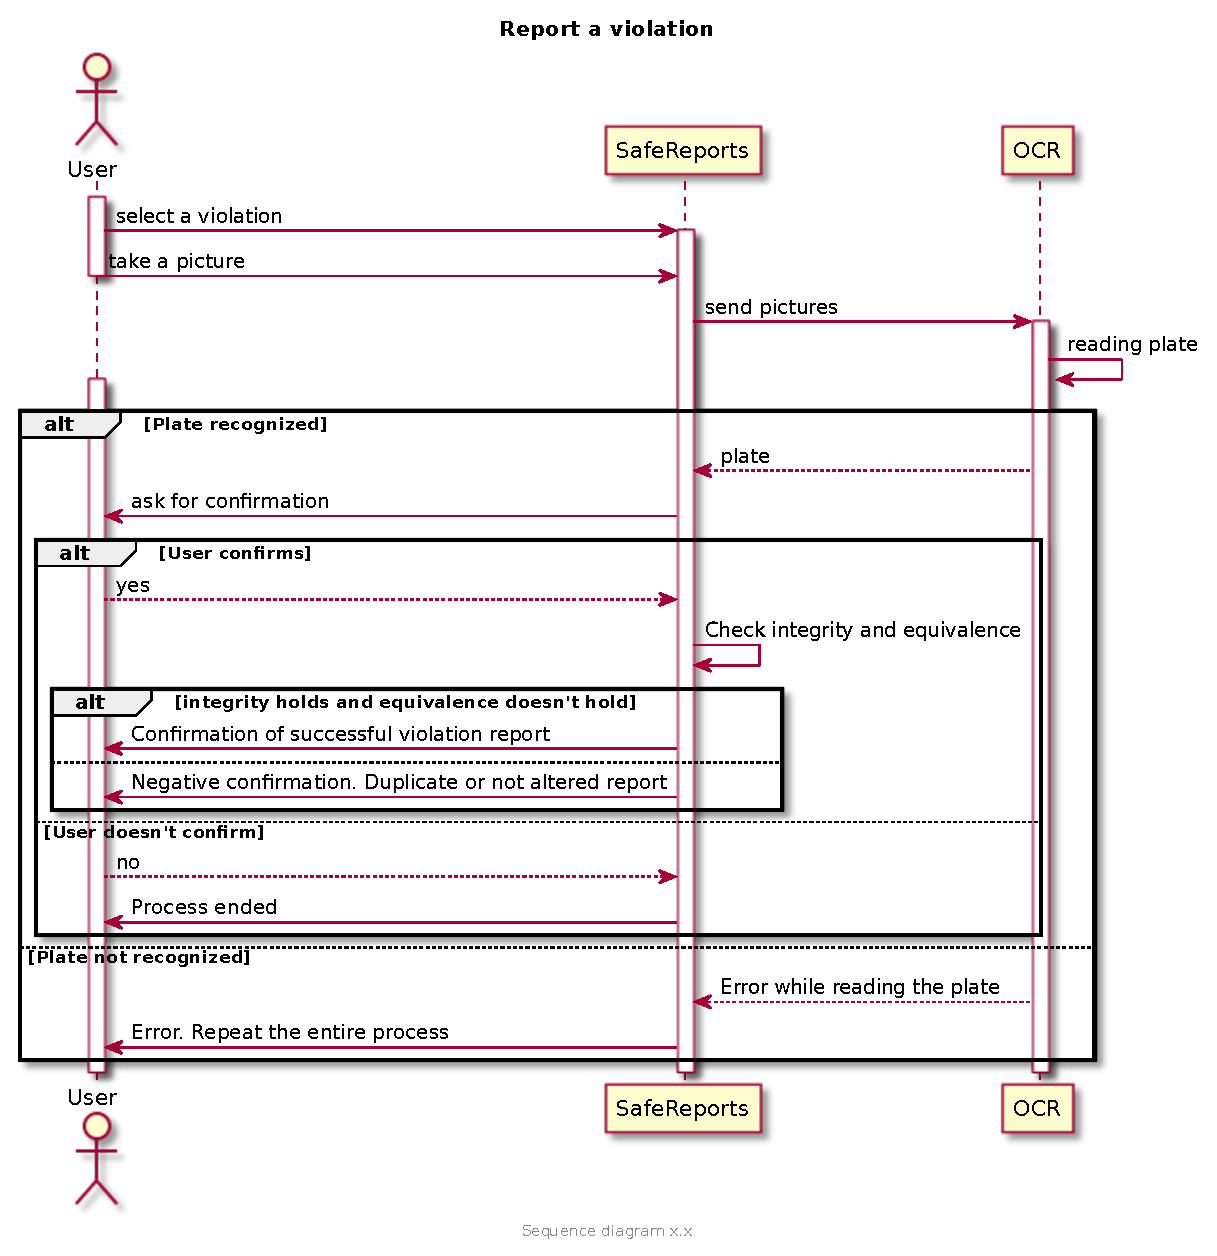
\includegraphics[width=\textwidth]{sequence_diagram_report}
\caption{Report a violation}
\end{figure}

\begin{figure}[H]
\centering
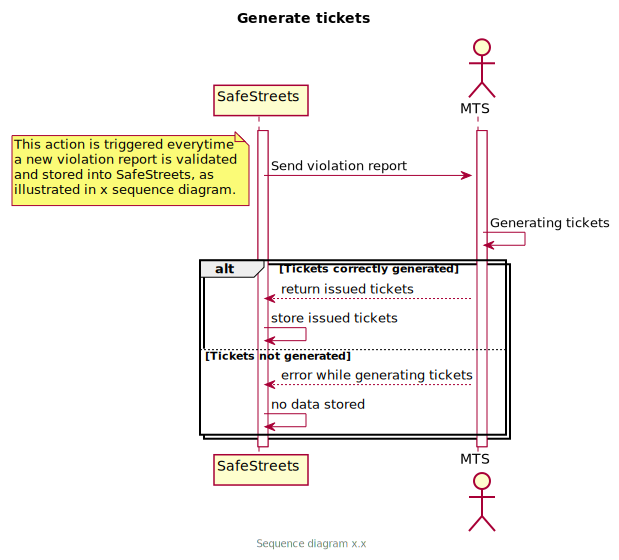
\includegraphics[width=0.85\textwidth]{sequence_tickets_generation}
\caption{Generate tickets}
\end{figure}

\begin{figure}[H]
\centering
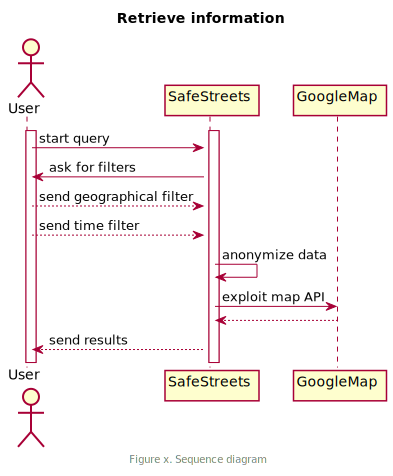
\includegraphics[width=0.55\textwidth]{sequence_diagram_retrieve_information}
\caption{Retrieve information}
\end{figure}

\subsubsection{Authorities}

\begin{figure}[H]
\centering
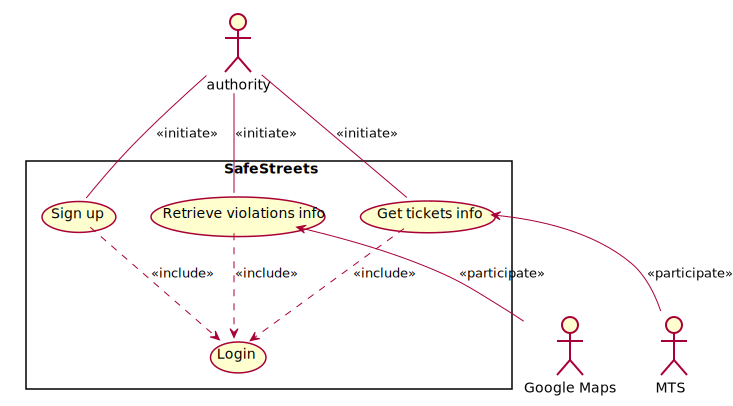
\includegraphics[width=\textwidth]{authorities_usecases}
\caption{Use cases diagram}
\end{figure}

\begin{table}[H]
\centering
\begin{tabularx}{\textwidth}{|l|X|}
\hline
Name & Sign up\tabularnewline
\hline
Actors &
\begin{itemize}[nosep,leftmargin=*]
\item Authority
\end{itemize}
\tabularnewline
\hline
Entry conditions &
\begin{itemize}[nosep,leftmargin=*]
\item The authority opens SafeStreets on his device
\end{itemize}
\tabularnewline
\hline
Events flow &
\begin{itemize}[nosep,leftmargin=*]
\item The authority chooses the sign up option
\item The authority selects the option to identify himself as authority
\item The authority inserts the activation code
\item The authority inserts his email and password
\item Authority confirms his data
\item SafeStreets saves his data
\end{itemize}
\tabularnewline
\hline
Exit conditions &
\begin{itemize}[nosep,leftmargin=*]
\item The authority is registered and his data are saved
\end{itemize}
\tabularnewline
\hline
Exceptions &
\begin{itemize}[nosep,leftmargin=*]
\item An account with the same email was already created. In this case
SafeStreets warns the authority and asks to change email or log in
\item The activation code is not valid. The authority is asked to reinsert
it
\item The authority doesn't provide all the data. In this case the system
asks him to insert them
\end{itemize}
\tabularnewline
\hline
\end{tabularx}
\end{table}

\begin{table}[H]
\centering
\begin{tabularx}{\textwidth}{|l|X|}
\hline
Name & Login\tabularnewline
\hline
Actors &
\begin{itemize}[nosep,leftmargin=*]
\item Authority
\end{itemize}
\tabularnewline
\hline
Entry conditions &
\begin{itemize}[nosep,leftmargin=*]
\item The authority has opened the application on his device
\item The authority is already registered
\end{itemize}
\tabularnewline
\hline
Events flow &
\begin{itemize}[nosep,leftmargin=*]
\item The authority chooses the login option
\item The authority inserts his email and password
\end{itemize}
\tabularnewline
\hline
Exit conditions &
\begin{itemize}[nosep,leftmargin=*]
\item The authority is identified
\end{itemize}
\tabularnewline
\hline
Exceptions &
\begin{itemize}[nosep,leftmargin=*]
\item The email is not registered. The authority is asked to reinsert it
or sign up
\item The password is incorrect. The authority is asked to reinsert it
\end{itemize}
\tabularnewline
\hline
\end{tabularx}
\end{table}

\begin{table}[H]
\centering
\begin{tabularx}{\textwidth}{|l|X|}
\hline
Name & Retrieve violation info\tabularnewline
\hline
Actors &
\begin{itemize}[nosep,leftmargin=*]
\item Authority
\item Google Maps
\end{itemize}
\tabularnewline
\hline
Entry conditions &
\begin{itemize}[nosep,leftmargin=*]
\item The authority is logged in SafeStreets
\item The authority wants to collect data about violations
\end{itemize}
\tabularnewline
\hline
Events flow &
\begin{itemize}[nosep,leftmargin=*]
\item The authority accesses the SafeAnalytics function
\item The authority selects the geographical filters
\item The authority selects the time filters
\item The authority selects the license plate filters
\item Data requested are sent to the authority
\end{itemize}
\tabularnewline
\hline
Exit conditions &
\begin{itemize}[nosep,leftmargin=*]
\item SafeStreets displays the data. If a map is required, it is provided
by Google Maps
\end{itemize}
\tabularnewline
\hline
Exceptions & -\tabularnewline
\hline
\end{tabularx}
\end{table}

\begin{table}[H]
\centering
\begin{tabularx}{\textwidth}{|l|X|}
\hline
Name & Get tickets info\tabularnewline
\hline
Actors &
\begin{itemize}[nosep,leftmargin=*]
\item Authority
\item MTS
\end{itemize}
\tabularnewline
\hline
Entry conditions &
\begin{itemize}[nosep,leftmargin=*]
\item The authority is logged in SafeStreets
\item The authority wants to get information about tickets issued by
SafeStreets
\end{itemize}
\tabularnewline
\hline
Events flow &
\begin{itemize}[nosep,leftmargin=*]
\item Authority accesses the SafeTickets functionality
\item The authority selects the geographical filters
\item The authority selects the time filters
\item The authority selects the license plate filters
\item Data requested are sent by SafeStreets to the authority
\end{itemize}
\tabularnewline
\hline
Exit conditions &
\begin{itemize}[nosep,leftmargin=*]
\item Safestreets displays the data
\end{itemize}
\tabularnewline
\hline
Exceptions & -\tabularnewline
\hline
\end{tabularx}
\end{table}

\begin{figure}[H]
\centering
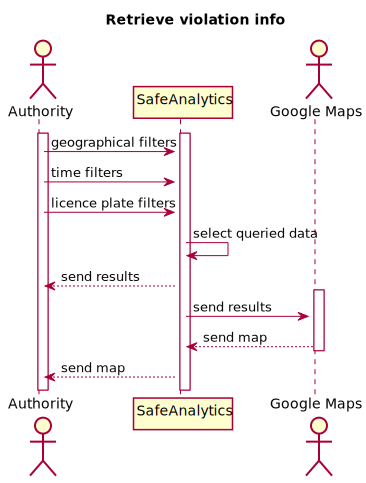
\includegraphics[width=0.65\textwidth]{retrieve_violation_info_sequence_diagram}
\caption{Retrieve violation info}
\end{figure}

\subsubsection{Municipality users}

\begin{figure}[H]
\centering
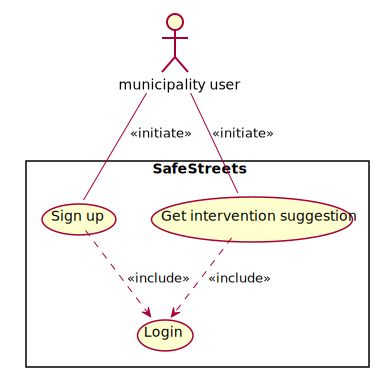
\includegraphics[width=\textwidth]{municipality_usecases}
\caption{Use cases diagram}
\end{figure}

\begin{table}[H]
\centering
\begin{tabularx}{\textwidth}{|l|X|}
\hline
Name & Get intervention suggestion\tabularnewline
\hline
Actors &
\begin{itemize}[nosep,leftmargin=*]
\item Municipality user
\end{itemize}
\tabularnewline
\hline
Entry conditions &
\begin{itemize}[nosep,leftmargin=*]
\item The municipality user has opened the application on his device and
logged in
\item The municipality user wants to get suggestions about possible
improvements
\end{itemize}
\tabularnewline
\hline
Events flow &
\begin{itemize}[nosep,leftmargin=*]
\item The municipality user accesses the SafeSuggestions functionality
\item The municipality user selects the geographical filters
\item SafeSuggestions gets possible interventions based on the filters
provided
\item SafeStreets sends (if available) the suggestion relative to the
filters provided
\end{itemize}
\tabularnewline
\hline
Exit conditions &
\begin{itemize}[nosep,leftmargin=*]
\item SafeStreets displays the suggestion (if given) or a "no suggestions"
notice
\end{itemize}
\tabularnewline
\hline
Exceptions & -\tabularnewline
\hline
\end{tabularx}
\end{table}

\begin{table}[H]
\centering
\begin{tabularx}{\textwidth}{|l|X|}
\hline
Name & Get accidents\tabularnewline
\hline
Actors &
\begin{itemize}[nosep,leftmargin=*]
\item Municipality
\end{itemize}
\tabularnewline
\hline
Entry conditions &
\begin{itemize}[nosep,leftmargin=*]
\item Timeout trigger is activated
\end{itemize}
\tabularnewline
\hline
Events flow &
\begin{itemize}[nosep,leftmargin=*]
\item New data is requested by SafeStreets from the municipality
\item The municipality evaluates if updates in data occurred
\item The municipality provides the new data to SafeStreets
\item Safestreets updates its data and builds new statistics in order to
generate new suggestions
\end{itemize}
\tabularnewline
\hline
Exit conditions &
\begin{itemize}[nosep,leftmargin=*]
\item The new suggestions are stored in the system
\end{itemize}
\tabularnewline
\hline
Exceptions & -\tabularnewline
\hline
\end{tabularx}
\end{table}

The use cases "Sign up" and "Login" are equal to the ones of the
authorities, and are omitted to avoid redundancies.

\begin{figure}[H]
\centering
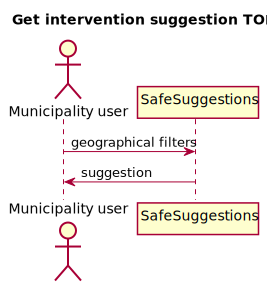
\includegraphics[width=0.7\textwidth]{get_intervention_suggestion_sequence_diagram}
\caption{Get intervention suggestion}
\end{figure}

\begin{figure}[H]
\centering
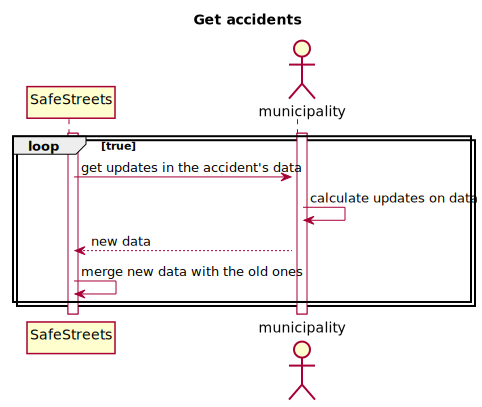
\includegraphics[width=0.9\textwidth]{get_accidents_sequence_diagram}
\caption{Get accidents}
\end{figure}

\subsubsection{Activities}

\begin{figure}[H]
\centering
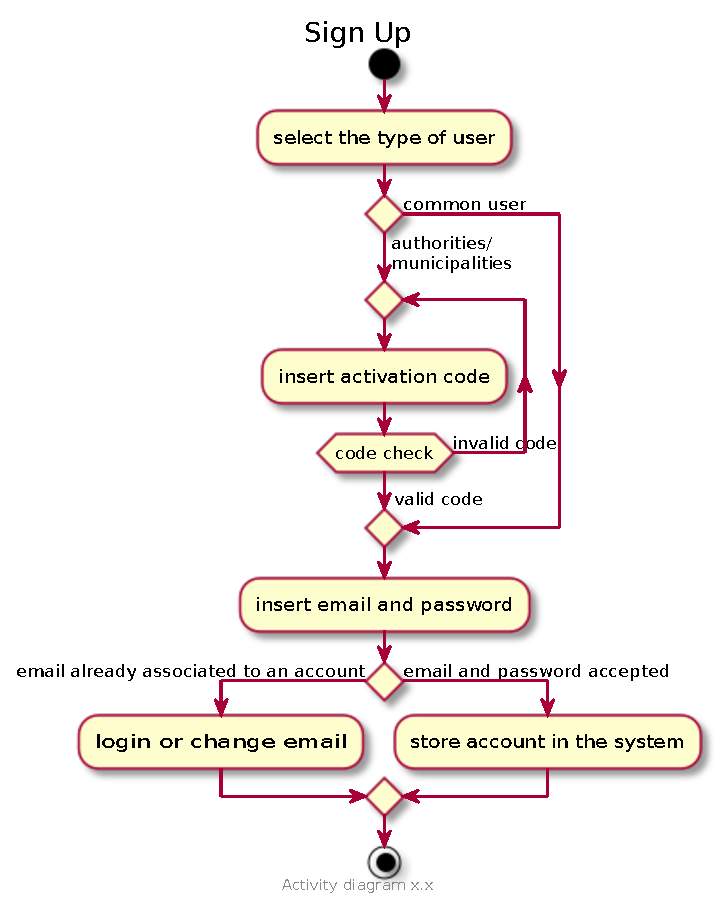
\includegraphics[width=\textwidth]{activity_diagram_login}
\caption{Registration}
\end{figure}

\begin{figure}[H]
\centering
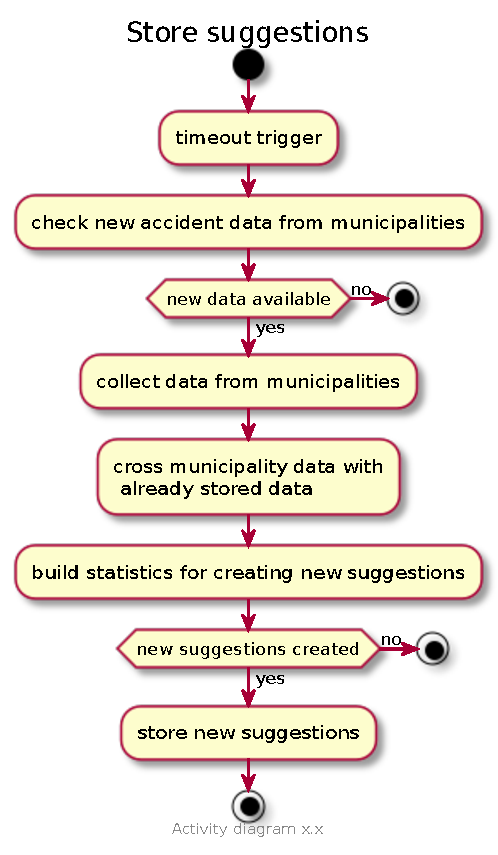
\includegraphics[width=0.7\textwidth]{activity_diagram_create_suggestions}
\caption{Generation of new suggestions}
\end{figure}

\subsubsection{Requirements}

\textbf{G1) SafeReports must allow common users to send violation
reports.}

\begin{itemize}
\item
  \textbf{R1} When a picture is taken using SafeReports, a new violation
  record is generated.
\item
  \textbf{R2} When a new violation record is generated, the current
  position of the user is added to the report.
\item
  \textbf{R3} When a new violation record is generated, the timestamp is
  added to the report.
\item
  \textbf{R4} When a new violation record is generated, the photo is
  scanned by an OCR software to automatically detect the plate.
\item
  \textbf{R5} If the OCR software fails in detecting the plate, the user
  is notified and asked to repeat the procedure.
\item
  \textbf{R6} If the OCR software detects the plate, the user is asked
  to confirm the violation report.
\item
  \textbf{R7} If the user confirms the violation report, it is sent to
  SafeStreets.
\item
  \textbf{R8} SafeStreets stores the information about the violation
  only if there aren't equivalent events already stored.
\end{itemize}

\textbf{G2) SafeAnalytics must allow common users to get anonymous data
on violations.}

\begin{itemize}
\item
  \textbf{R9} SafeAnalytics allows common users to get data about
  violations selecting zone, time and type of violation.
\item
  \textbf{R10} SafeAnalytics anonymizes information before sending it to
  common users.
\end{itemize}

\textbf{G3) SafeAnalytics must allow authorities to access to all the
data without restrictions.}

\begin{itemize}
\item
  \textbf{R11} SafeAnalytics allows authorities to get all the information
  stored by SafeStreets.
\end{itemize}

\textbf{G4) SafeSuggestions must allow municipality users to get
suggestions on possible interventions.}

\begin{itemize}
\item
  \textbf{R12} SafeStreets must store data about accidents provided by
  the municipality when available.
\item
  \textbf{R13} SafeStreets must analyze collected data crossed with data
  from the municipality to identify possible interventions.
\item
  \textbf{R14} SafeSuggestions allows municipality users to get
  suggestions provided by SafeStreets.
\end{itemize}

\textbf{G5) SafeStreets must generate traffic tickets forwarding
reliable data to MTS.}

\begin{itemize}
\item
  \textbf{R15} When the users send a violation report, its integrity is
  checked.
\item
  \textbf{R16} If the integrity check is not successful, the violation
  report is discarded.
\item
  \textbf{R17} SafeStreets must forward every new stored violation
  report to MTS to generate traffic tickets.
\end{itemize}

\textbf{G6) SafeTickets must allow authorities to get statistics on
issued tickets.}

\begin{itemize}
\item
  \textbf{R18} When a new ticket is generated using MTS, ticket-related
  data are stored by SafeStreets.
\item
  \textbf{R19} SafeStreets must build statistics from stored data about
  issued tickets.
\item
  \textbf{R20} SafeTickets allows authorities to get information and
  statistics on issued tickets.
\end{itemize}

\subsubsection{Traceability matrix}

\begin{table}[H]
\centering
\begin{tabular}{|l|l|l|}
\hline
Requirements & Goal & Use case\tabularnewline
\hline
R1 & G1 & Report violations\tabularnewline
R2 & G1 & Report violations\tabularnewline
R3 & G1 & Report violations\tabularnewline
R4 & G1 & Report violations\tabularnewline
R5 & G1 & Report violations\tabularnewline
R6 & G1 & Report violations\tabularnewline
R7 & G1 & Report violations\tabularnewline
R8 & G1 & Report violations\tabularnewline
R9 & G2 & Retrieve information\tabularnewline
R10 & G2 & Retrieve information\tabularnewline
R11 & G3 & Retrieve violations info\tabularnewline
R12 & G4 & Get accidents\tabularnewline
R13 & G4 & Get accidents\tabularnewline
R14 & G4 & Get intervention suggestion\tabularnewline
R15 & G5 & Generate tickets\tabularnewline
R16 & G5 & Generate tickets\tabularnewline
R17 & G5 & Generate tickets\tabularnewline
R18 & G6 & Generate tickets\tabularnewline
R19 & G6 & Generate tickets\tabularnewline
R20 & G6 & Get tickets info\tabularnewline
\hline
\end{tabular}
\end{table}

\subsection{Performance Requirements}

\begin{itemize}
\item
  The system must be able to serve a great number of users reporting a
  violation simultaneously.
\item
  SafeAnalytics must be able to provide the data requested by both
  common users and authorities in less than 3 seconds, to provide the
  best experience.
\item
  The data about accidents provided by the municipality must be checked
  for updates at least every 5 minutes, to provide reliable and always
  updated suggestions.
\end{itemize}

\subsection{Design Constraints}

\subsubsection{Standards compliance}

The timestamp must adopt the ISO 8601 standard. The chain of custody of
the information coming from the user must never be broken, so the
correspondence of the data provided by a common user and the one
received by MTS must be guaranteed.

\subsubsection{Hardware limitations}

To correctly run the application, the device must have a camera with a
resolution sufficient to provide an understandable image, a working
internet connection, and a GPS.

\subsubsection{Any other constraint}

The system must not provide sensitive data to common users, so the
license plate and the photo of a violation must not be provided to them.

\subsection{Software System Attributes}

\subsubsection{Reliability}

SafeStreets must be fault-tolerant, so data must not be lost. This can
be achieved by keeping multiple copies of the data.

\subsubsection{Availability}

SafeStreets must be working 24/7.\\
SafeReports is expected to work with an availability of 99.999\%, as it
is the core of the application. The other functionalities can be
slightly less fault-tolerant, and be available 99.99\% of the time.

\subsubsection{Security}

The data provided by common users contain sensitive information, so
security is a crucial point. The databases on which data is collected
must be protected to avoid attacks, and the software must be GDPR
compliant. Data must be encrypted when sent, and the reliability of the
data received by MTS must be checked.

\subsubsection{Maintainability}

The code must be easy to fix and modify, to reduce the effort and the
cost of the modifications. It must avoid fast obsolescence, so be always
as aligned as possible to the new stable technologies.\\
The modularity of the code and the reusability of the logic (which needs
to be as separated as possible from the implementation) are needed to
guarantee the ease of maintenance in the future.

\subsubsection{Portability}

The software is thought to run on the majority of mobile devices, so it
should be developed for Android and iOS smartphones.

\end{document}